\en

\section{Refactoring}

Fowler defines refactoring in his book as "a controlled technique for improving the design of an existing code base. 
Its essence is applying a series of small behavior-preserving transformations, each of which is too small to be worth 
doing. However, the cumulative effect of each of these transformations is quite significant." \citep{refactorbook}. 
The elimination of detected code clone duplication is a refactoring task that necessitates the 
application of refactoring methods. Fowler presents multiple refactoring methods such as the 
\textit{parameterize method}, the \textit{replace parameter with explicit methods} and 
the \textit{replace parameter with method} \citep{refactorbook}. 
There is a brief explanation of the methods used in our research below.

\paragraph{Parameterize method}

\

The Parameterize method consists of replacing multiple similar codes with a singular function. 
The function created implements the different behaviors between similar codes by using parameters, 
which tell which behavior the function should use \citep{refactorbook}.
Figure \ref{fig:parameter} demonstrates an example of the Parameterize method usage.

\begin{figure}
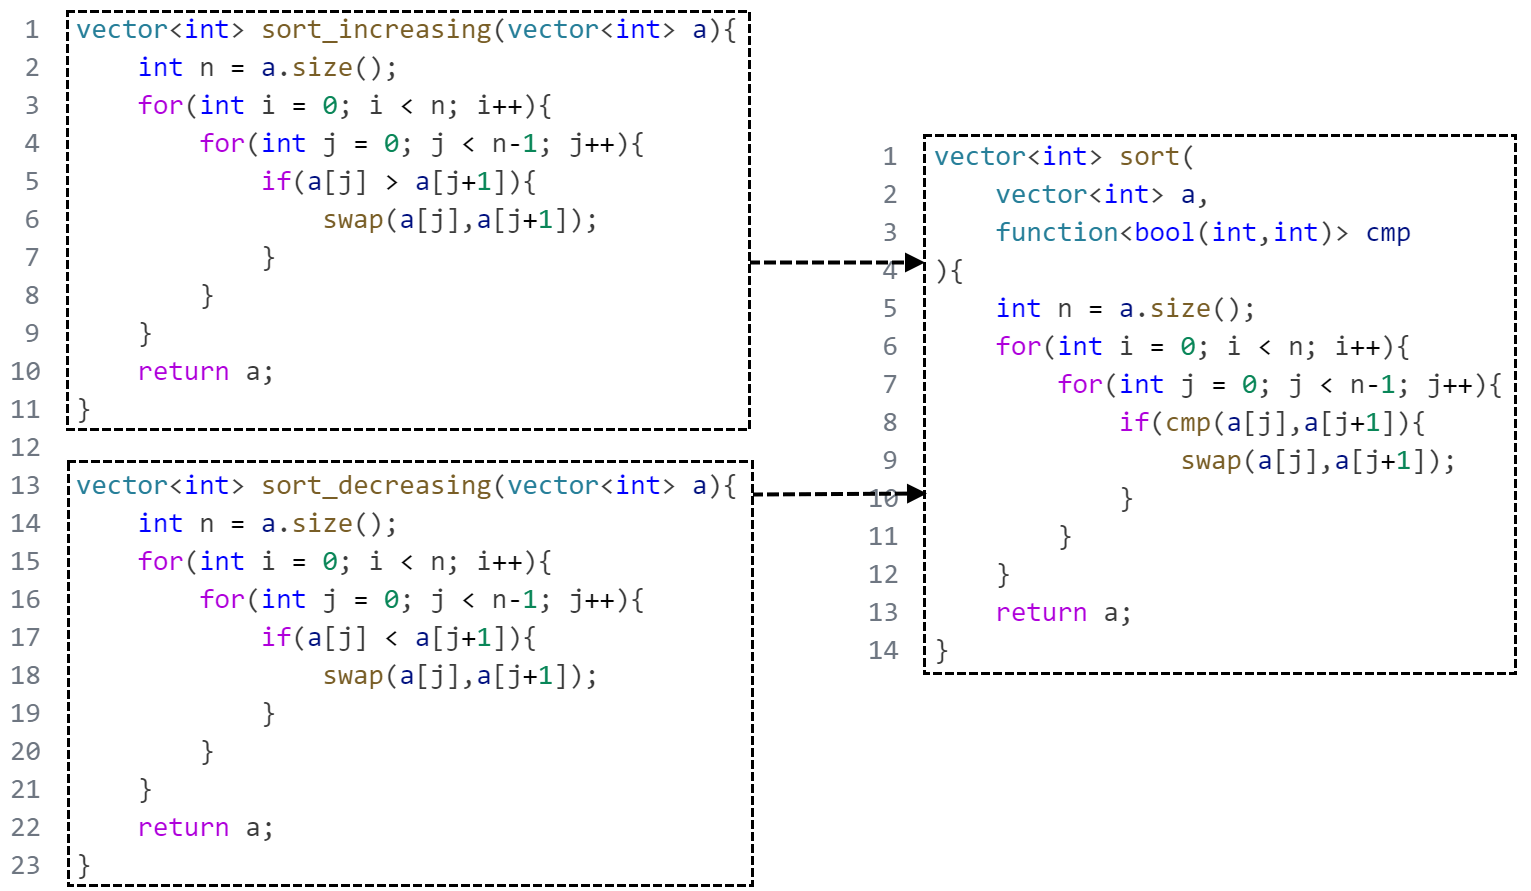
\includegraphics[scale=0.36]{refactor/parameterize}
\caption{Example of Parameterize method usage.}
\label{fig:parameter}
\end{figure}


\paragraph{Extract method}

\

The Extract method consists of splitting a complex code artifact into multiple simple methods/functions. 
One of the advantages of this method is enabling the created functions to be used multiple times through 
the code project. In contrast, with only the complex code artifact, it is not always possible to reuse 
it entirely, thus creating a new code duplication \citep{refactorbook}. 
Figure \ref{fig:extract} demonstrates an example of the Extract method usage.

\begin{figure}
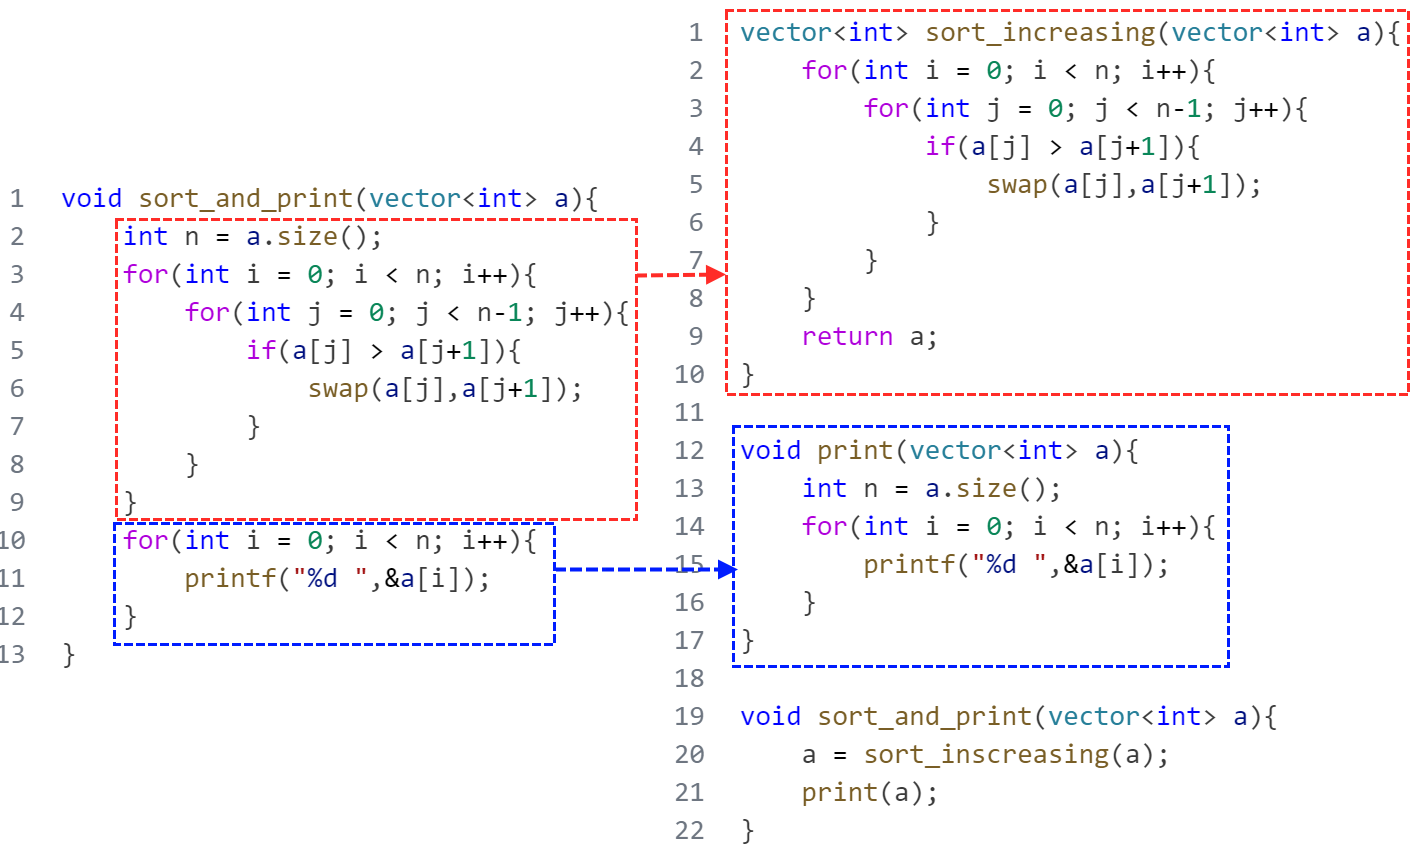
\includegraphics[scale=0.36]{refactor/extract}
\caption{Example of Extract method usage.}
\label{fig:extract}
\end{figure}

